% Official CVPR 2027 review format; template hashes are in README.md.
\documentclass[10pt,twocolumn,letterpaper]{article}
\ifdefined\XeTeXversion
  \usepackage[OT1]{fontenc}
\fi
\usepackage[review]{cvpr}
\usepackage{amsmath,amssymb,booktabs,graphicx}
\definecolor{cvprblue}{rgb}{0.21,0.49,0.74}
\usepackage[pagebackref,breaklinks,colorlinks,allcolors=cvprblue]{hyperref}
\def\confName{CVPR}
\def\confYear{2027}
\newcommand{\pending}{\phantom{0.000}}
\newcommand{\ours}{Demodulation-first}
\title{Demodulate, Then Attend:\\Exposing Amplitude Dynamics for Compact EEG Models}
\author{}
\begin{document}
\maketitle

\begin{abstract}
Modern electroencephalography (EEG) models increasingly rely on larger
networks and more pretraining. We revisit a simpler choice: the signal
representation on which learning operates.
We advocate demodulation before attention: extract each band's amplitude
envelope and pair it with the corresponding waveform, exposing both
amplitude dynamics and oscillatory morphology.
Scattering theory motivates this separation and explains why temporal
averaging can discard useful modulation structure.
A simple tokenizer applies a learnable filterbank and embeds matched
local waveform and envelope sequences into an electrode--band--time grid.
A compact axial Transformer reads this representation.
With the reader and training recipe fixed, this representation improves
TUEV Cohen's $\kappa$ from 0.576 to 0.711, an absolute gain of 0.135,
while using fewer parameters; the same construction achieves 0.699 PR-AUC
on CHB-MIT with 1.62 million parameters and no pretraining.
With the filterbank and reader unchanged, waveform-only and envelope-only
tokens reach 0.498 and 0.642 on TUEV, compared with 0.711 for the pair.
These results motivate a representation-first approach to compact EEG
models: make useful signal structure available in the tokens, then learn
how it is organized across time, electrodes, and frequency.
\end{abstract}

\begin{figure*}[t]
  \centering
  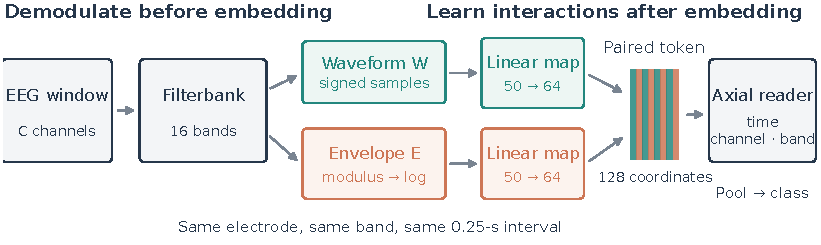
\includegraphics[width=\textwidth]{figures/architecture.pdf}
  \caption{\textbf{Demodulate, then attend.} A learned filterbank produces
  band-limited waveforms. The analytic modulus supplies a corresponding
  amplitude envelope. Shared projections embed both 50-sample sequences
  into one token, retaining their electrode, band, and time indices.
  Six axial Transformer blocks learn interactions on this grid. The
  analytic transform is applied to the full input window before patching.}
  \label{fig:architecture}
\end{figure*}

\section{Introduction}
\label{sec:intro}
EEG modeling has progressed from compact convolutional networks to
Transformers pretrained on large collections of recordings
\citep{schirrmeister2017deep,lawhern2018eegnet,jiang2024labram,wang2025cbramod}.
Yet larger models do not consistently
outperform compact supervised specialists \citep{liu2026compass}.
This observation motivates a more basic question: what representation
should an EEG model learn from? We examine the signal computations
performed before attention and the signal properties they expose.

Clinical EEG descriptions characterize morphology, recurrence, evolution, and
spatial distribution \citep{hirsch2021acns}. A sharp discharge and a
smooth oscillation differ in waveform shape; sustained activity and
separated bursts differ in how their strength evolves. These properties
motivate two descriptions of each frequency band. The signed
\emph{waveform} retains oscillatory shape, while the amplitude
\emph{envelope} tracks how activity strengthens and weakens. Their
correspondence matters: a transient has a local shape and occurs within
an evolving pattern of activity.

These two descriptions suggest a concrete input choice. Raw-patch
embedding leaves the envelope implicit: exposing bandwise amplitude
requires filtering followed by a nonlinear modulus, which a linear patch
projection cannot compute. Supplying an envelope performs this operation
before learning, but removes polarity and phase detail. We therefore
retain the corresponding signed waveform and ask whether the two views
are more useful together than either alone. This leads to
\emph{demodulation before attention}: expose amplitude dynamics without
replacing the waveform that carries them. We hypothesize that this input
choice simplifies a compact encoder's learning problem.

Scattering theory clarifies what should be preserved after demodulation.
Bandpass transforms and modulus operations expose subband amplitude,
but subsequent averaging can discard temporal modulation structure
\citep{anden2014scattering}. An envelope trajectory can distinguish
burst patterns with similar average band energy.
At the same time, taking a modulus discards waveform polarity and phase
detail. These observations motivate preserving the envelope sequence
together with its signed waveform: demodulation exposes a useful view
of the signal without making that view the entire representation.

The resulting tokenizer is simple. A learnable filterbank decomposes
each channel into bands, and an analytic transform extracts their
envelopes before patching. Shared projections pair waveform and
log-envelope sequences from the same electrode, band, and interval. The
tokens form an electrode--band--time grid, read by an ordinary axial
Transformer. Attention relates intervals along time, locations across
channels, and components across bands. The complete model is trained
with supervised classification alone.

Frequency-aware frontends provide important precedents. CBraMod adds
patchwise spectral and convolutional waveform features
\citep{wang2025cbramod}. TFM-Tokenizer learns discrete motifs from
waveform and time--frequency representations
\citep{pradeepkumar2026tfm}. The Morlet Spectral Transformer preserves
time-resolved wavelet amplitudes \citep{qing2026morlet}.
We study a specific continuous input representation: the local pairing
of a band's waveform and envelope trajectory before attention.
Holding the reader fixed makes it possible to compare this explicit
signal representation with raw learned rows, and to separate the
contributions of its two content views through controlled replacements.

The reference reaches $\kappa=0.711$ on TUEV and PR-AUC 0.699
on CHB-MIT using 1.62 million parameters. On TUEV, replacing it with raw
patches projected into the same number of learned rows reduces $\kappa$
to 0.576 under the same reader, split, and training recipe: an absolute
difference of 0.135 with fewer parameters in the proposed model.
Holding the filterbank fixed further separates the two content views:
waveform-only and envelope-only tokens reach 0.498 and 0.642,
respectively, while their pairing reaches 0.711. F1 improves in all six
event categories in the raw-row comparison. A separate linear readout
of frozen tokens checks that both intended trajectories remain available
before attention.

We propose demodulation before attention as a simple principle for EEG
tokenization, implement it with local waveform--envelope pairs, and
examine its effect with a fixed compact reader. The resulting model
connects an explicit signal representation to clinical prediction
without a separate pretraining stage. More broadly, this work asks
which useful signal computations should precede learning, so that an
encoder can build on directly available structure in the recording.

\section{Related Work}
\label{sec:related}
\subsection{EEG pretraining and tokenization}
EEG foundation models address transfer across subjects, tasks, and
recording systems. BIOT organizes channelwise signal segments into a
common sequence \citep{yang2023biot}. LaBraM learns discrete neural codes
through spectrum prediction \citep{jiang2024labram}, and EEGPT uses
masked representation learning with alignment \citep{wang2024eegpt}.
CBraMod separates spatial and temporal interactions in a criss-cross
Transformer \citep{wang2025cbramod}; REVE extends large-scale pretraining
to heterogeneous acquisition setups \citep{elouahidi2025reve}.
These methods combine input representations, learning objectives, and
encoder designs to obtain transferable features.

TFM-Tokenizer instead makes the frontend a primary object of study:
waveform and spectral paths produce a vocabulary of time--frequency
motifs that can serve different encoders \citep{pradeepkumar2026tfm}.
Our construction uses continuous, explicitly demodulated band content.
It does not require a learned codebook or a separate tokenizer pretraining
stage. The question is which local signal views should remain available
inside each token before the encoder mixes information across locations.

\subsection{Amplitude-based EEG representations}
Explicit amplitude information is well established in EEG decoding.
The shallow network of Schirrmeister et al. uses squaring, pooling, and
logarithmic compression to extract power-related features
\citep{schirrmeister2017deep}. FBCNet combines a filterbank, spatial
filtering, and variance aggregation \citep{mane2021fbcnet}.
EEGNet provides another compact architecture through factorized temporal
and spatial filtering \citep{lawhern2018eegnet}.
HTNet computes filter--Hilbert power at learned frequencies before neural
decoding \citep{Peterson_2021}. Hilbert envelopes and temporal fine
structure have also been concatenated for EEG speech decoding
\citep{duraisamy2025transferlearningcovertspeech}.

Recent frontends also preserve spectral or amplitude variation.
CBraMod projects a one-second patch spectrum and combines it with
waveform features \citep{wang2025cbramod}. The Morlet Spectral Transformer
uses wavelet modulus, temporal pooling, and frequency-specific spatial
projections \citep{qing2026morlet}. Our distinction is narrower than
introducing amplitude: a token embeds a sequence of envelope samples and
the corresponding signed waveform from one band, while electrodes remain
a token axis. This makes local content and the granularity of its
representation explicit experimental variables.

\subsection{Demodulation before learned processing}
The deep scattering spectrum extracts subband envelopes with analytic
wavelets and modulus operations, then recovers modulation structure that
would be lost through averaging \citep{anden2014scattering}. We adopt
the demodulation principle while passing local trajectories to learned
attention. The implementation uses trainable sinc filters
\citep{ravanelli2018sincnet}, rather than a fixed scattering cascade.
Its contribution is the token interface, not a new demodulation theorem.

\section{Method}
\label{sec:method}
Let $x_c[t]$ be the normalized EEG signal at channel $c$. We construct
one token per channel $c$, band $b$, and time interval $p$. The method
has three steps: demodulate the bands, embed paired local content, and
read the resulting grid (\cref{fig:architecture}).

\subsection{Bandwise demodulation}
\label{sec:demod}
A shared bank of $B$ learnable bandpass filters produces signed
waveforms $w_{c,b}$ and their analytic envelopes:
\begin{equation}
  \begin{aligned}
    w_{c,b}&=g_b*x_c,\\
    e_{c,b}&=\big|w_{c,b}+\mathrm{i}\mathcal{H}[w_{c,b}]\big|.
  \end{aligned}
  \label{eq:demod}
\end{equation}
where $\mathcal{H}$ is the Hilbert transform. Each sinc filter $g_b$
is parameterized by two cutoffs \citep{ravanelli2018sincnet}. We use
16 filters, initialized with logarithmically spaced edges from
0.5 to 75 Hz, and a 201-sample impulse response at 200 Hz. The cutoffs
are learned during supervised training.

For a narrowband amplitude-modulated component
$w(t)=A(t)\cos\phi(t)$ with suitable separation between modulation and
carrier frequencies, the analytic envelope approximates $A(t)$.
Thus the modulus exposes amplitude dynamics that would otherwise need
to be derived from oscillating samples. With general EEG, it is the
well-defined amplitude of the filtered analytic signal; it need not
identify a single physiological oscillator. We retain the signed
waveform in parallel because taking a modulus removes its phase and
polarity information.

Filtering and the analytic transform operate on the entire input window.
Only afterward do we divide the two sequences into tokens. A 0.25-s
token therefore summarizes a local part of an envelope estimated with
context beyond that token. The token interval is not the filter's
support and does not impose a 0.25-s Hilbert-estimation window.

\subsection{Pair local waveform and envelope trajectories}
\label{sec:token}
For interval $p$ of length $L$, let
$\mathbf{w}_{c,b,p}\in\mathbb{R}^{L}$ and
$\mathbf{e}_{c,b,p}\in\mathbb{R}^{L}$ contain corresponding waveform
and envelope samples. We form
\begin{equation}
  \mathbf{h}_{c,b,p}
  =\left[
     P_E\log(1+\mathbf{e}_{c,b,p})+\mathbf{b}_E\,;\,
     P_W\mathbf{w}_{c,b,p}
    \right],
  \label{eq:token}
\end{equation}
with $P_E,P_W\in\mathbb{R}^{(d/2)\times L}$.
Both projections are shared across channels, bands, and intervals.
The implementation interleaves the two sets of coordinates, which is
a fixed permutation of the concatenation in \cref{eq:token}.
We use $L=50$ and $d=128$. The logarithm compresses envelope dynamic
range without averaging its trajectory.

The pairing is deliberately local. Each token places waveform and
amplitude dynamics from the same signal component in a common learned
representation. The encoder can then model their relationship without
first matching independently aggregated views. We preserve all 50 input
positions through separate projections rather than substituting a
single power or variance statistic. There is no phase rotation or
additional learned fusion module at this stage.

This construction also separates \emph{available information} from
\emph{explicit computation}. A raw-patch projection can preserve all its
input samples when its matrix has sufficient rank. It nevertheless does
not output an amplitude envelope: the modulus is nonlinear. Our design
supplies this computation before attention and retains the waveform from
which it was derived. It introduces a representational bias, not an
additional measurement of the underlying EEG.

\subsection{A compact reader for the token grid}
\label{sec:reader}
Tokens form a $C\times B\times P$ grid. Channel embeddings derived
from electrode coordinates and learned band-index embeddings identify
the two non-temporal axes. Each pre-normalized Transformer block applies
self-attention along time, channels, and bands in sequence, followed by
a feed-forward network. Time attention uses rotary positions. Each axis
uses ordinary four-head attention; the reference has six blocks,
width 128, and a feed-forward expansion of two.

The axes follow the representation: time relates intervals, channels
relate recording locations, and bands relate signal components.
Factorization permits this grid to be read without global attention
over all its tokens. Global mean pooling, layer normalization, and a linear classifier
predict the window label. The complete reference
contains approximately 1.62 million parameters. We keep this reader
fixed in the content experiments; it is not a separate proposed
attention mechanism.

\begin{figure}[t]
  \centering
  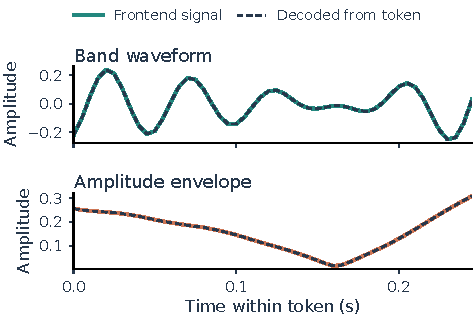
\includegraphics[width=\columnwidth]{figures/recovery.pdf}
  \caption{\textbf{What remains in a token?} A linear readout of frozen
  TUEV tokens recovers the waveform and envelope of a held-out band
  segment. Curves overlap at this scale. This checks local content
  preservation before attention; classification controls test utility.}
  \label{fig:recovery}
\end{figure}

\begin{table}[t]
  \centering
  \caption{\textbf{Content recovery before attention.} Held-out normalized
  RMSE of linear readouts fitted to frozen tokens. Targets are the
  frontend's waveform and log-envelope samples.}
  \label{tab:recovery}
  \small
  \begin{tabular}{lcc}
    \toprule
    Target & TUEV & CHB-MIT \\
    \midrule
    Waveform & $3.21\!\times\!10^{-4}$ & $1.33\!\times\!10^{-4}$ \\
    Log-envelope & $4.13\!\times\!10^{-7}$ & $5.38\!\times\!10^{-7}$ \\
    \bottomrule
  \end{tabular}
\end{table}

\subsection{Checking the token's content}
\label{sec:recovery}
Before attributing a classification result to preserved content, we
check that the two intended views can be recovered from the token.
We freeze the trained frontend and fit separate linear readouts to
waveform and log-envelope samples, using training windows only. Readout
regularization is selected on validation windows; reconstruction is
measured on held-out test windows. No classification labels enter this
check, and no classifier weights are updated.

Both content views are recovered with small error
(\cref{tab:recovery,fig:recovery}). The two $64\times50$ projection
matrices have full column rank in both trained models, explaining why
linear recovery is possible. This is a functional check of the
representation, not evidence that every retained coordinate is needed
for classification. In particular, reconstruction does not establish
whether a waveform-only or envelope-only token would perform equally
well. Those questions require the content controls in \cref{sec:controls}.

\section{Experimental Setup}
\label{sec:setup}
\paragraph{Tasks and data.}
We study six-class event classification on TUEV
\citep{nedcTUEV} and binary seizure-window classification on CHB-MIT
\citep{guttag2010chbmit}. Both use 16 bipolar channels at 200 Hz.
TUEV contains 5-s event-centered windows, with subject-separated training
and validation sets drawn from the official training partition and the
official evaluation subjects reserved for testing. CHB-MIT uses 10-s
windows and case-separated partitions. Its evaluated protocol includes
additional seizure-centered windows in each partition; the test set has
17,386 windows, including 276 positives. All within-dataset comparisons
must use these same windows. Appendix~\ref{app:data} gives normalization,
partition counts, and the exact sampling protocol.

\paragraph{Training.}
The reference and content controls are trained from scratch with AdamW,
a learning rate of $10^{-4}$,
weight decay 0.05, cosine scheduling, batch size 32, and a maximum of
20 epochs. The configured dropout is 0.35. TUEV uses cross-entropy with
label smoothing 0.1; CHB-MIT uses focal loss with $\alpha=0.25$ and
$\gamma=2$. All content arms share the same data augmentation, optimizer,
reader, and checkpoint-selection rule. Appendix~\ref{app:recipe} details
the transformations and validation schedule.

\paragraph{Evaluation.}
We select checkpoints by validation $\kappa$ on TUEV and validation
PR-AUC on CHB-MIT. The held-out test set is used for reporting. TUEV
reports $\kappa$, balanced accuracy, and support-weighted F1. CHB-MIT
reports trapezoidal PR-AUC, AUROC, and balanced accuracy at threshold
0.5; we additionally give average precision. The reference and content controls use seed 2. Historical baseline
cells summarize seeds 0, 1, and 2 with sample SD, except the available
shared-protocol TUEV LaBraM and EEGPT runs, which use seed 0.
Baseline recipes and task adaptations are documented in
Appendix~\ref{app:baselines}. Empty cells have no compatible completed
run; scores from other montages or window sets are not substituted.

\begin{table*}[t]
  \centering
  \caption{\textbf{Clinical evaluation on shared data protocols.}
  Baselines reuse completed runs with their recorded task adaptations
  (Appendix~\ref{app:baselines}). Values with dispersion are mean $\pm$
  sample SD; single-run entries have no SD. Size gives recorded parameter
  counts in millions for TUEV / CHB-MIT; unrecorded counts are shown as
  --. Bold marks the highest available score in each column.}
  \label{tab:main}
  \small
  \setlength{\tabcolsep}{2.4pt}
  \begin{tabular}{lcrrrrrr}
    \toprule
    & & \multicolumn{3}{c}{TUEV} & \multicolumn{3}{c}{CHB-MIT} \\
    \cmidrule(lr){3-5}\cmidrule(lr){6-8}
    Model & Size (M) & $\kappa\uparrow$ & Bal. acc.$\uparrow$ & wF1$\uparrow$
    & PR-AUC$\uparrow$ & AUROC$\uparrow$ & Bal. acc.$\uparrow$ \\
    \midrule
    \multicolumn{8}{l}{\emph{Pretrained}} \\
    BIOT \citep{yang2023biot} & 3.19 / 3.19 & $0.530\!\pm\!0.028$ & $0.489\!\pm\!0.030$ & $0.753\!\pm\!0.016$ & $0.560\!\pm\!0.077$ & $0.874\!\pm\!0.004$ & $0.619\!\pm\!0.045$ \\
    LaBraM \citep{jiang2024labram} & -- / 5.82 & $0.602$ & $\boldsymbol{0.655}$ & $0.797$ & $0.452\!\pm\!0.097$ & $0.871\!\pm\!0.062$ & $0.586\!\pm\!0.047$ \\
    EEGPT \citep{wang2024eegpt} & -- / 25.69 & $0.634$ & $0.594$ & $0.812$ & $0.281\!\pm\!0.133$ & $0.857\!\pm\!0.038$ & $0.547\!\pm\!0.063$ \\
    CBraMod \citep{wang2025cbramod} & 17.85 / 30.65 & $0.645\!\pm\!0.022$ & $0.603\!\pm\!0.011$ & $0.813\!\pm\!0.012$ & $0.233\!\pm\!0.098$ & $0.783\!\pm\!0.047$ & $0.545\!\pm\!0.020$ \\
    REVE \citep{elouahidi2025reve} & 69.48 / 69.46 & $0.685\!\pm\!0.039$ & $0.648\!\pm\!0.018$ & $0.838\!\pm\!0.019$ & $0.580\!\pm\!0.196$ & $0.898\!\pm\!0.064$ & $0.632\!\pm\!0.068$ \\
    TFM-Tokenizer \citep{pradeepkumar2026tfm} & 1.89 / 1.89 & $0.652\!\pm\!0.021$ & $0.596\!\pm\!0.036$ & $0.817\!\pm\!0.010$ & $0.627\!\pm\!0.025$ & $\boldsymbol{0.929\!\pm\!0.006}$ & $\boldsymbol{0.634\!\pm\!0.016}$ \\
    \midrule
    \multicolumn{8}{l}{\emph{From scratch}} \\
    BIOT \citep{yang2023biot} & 3.19 / 3.19 & $0.532\!\pm\!0.025$ & $0.535\!\pm\!0.062$ & $0.761\!\pm\!0.013$ & $0.566\!\pm\!0.072$ & $0.875\!\pm\!0.019$ & $0.624\!\pm\!0.071$ \\
    LaBraM \citep{jiang2024labram} & -- / 5.82 & $0.569$ & $0.380$ & $0.766$ & $0.360\!\pm\!0.050$ & $0.823\!\pm\!0.030$ & $0.585\!\pm\!0.065$ \\
    EEGPT \citep{wang2024eegpt} & -- / -- & $0.578$ & $0.530$ & $0.783$ & \pending & \pending & \pending \\
    CBraMod \citep{wang2025cbramod} & 17.85 / 30.65 & $0.564\!\pm\!0.024$ & $0.574\!\pm\!0.010$ & $0.767\!\pm\!0.004$ & $0.317\!\pm\!0.205$ & $0.780\!\pm\!0.133$ & $0.602\!\pm\!0.088$ \\
    REVE \citep{elouahidi2025reve} & 69.48 / -- & $0.319\!\pm\!0.014$ & $0.370\!\pm\!0.042$ & $0.655\!\pm\!0.004$ & \pending & \pending & \pending \\
    \ours{} (ours) & 1.62 / 1.62 & $\boldsymbol{0.711}$ & $0.634$ & $\boldsymbol{0.849}$ & $\boldsymbol{0.699}$ & $0.918$ & $0.630$ \\
    \bottomrule
  \end{tabular}
\end{table*}

\section{Results}
\label{sec:results}
\subsection{Clinical performance}
The 1.62M reference achieves $\kappa=0.711$ on TUEV and PR-AUC 0.699
on CHB-MIT (\cref{tab:main}). It exceeds the highest recorded pretrained
baseline primary scores, from REVE and TFM-Tokenizer respectively, by
0.027 and 0.073. CHB-MIT average precision is 0.702, close to its
trapezoidal PR-AUC of 0.699.

To examine the frontend directly, we hold the reader and training recipe
fixed and change its input (\cref{tab:fixed-reader}). A linear map turns
each raw 50-sample channel patch into 16 learned rows of width 128,
matching the reference token grid. Replacing these rows with bandwise
waveform--envelope pairs improves all three metrics, including an
absolute $\kappa$ gain of 0.135, with fewer parameters. The comparison
tests the complete frontend; the content controls below separate its views.
On CHB-MIT, paired input raises PR-AUC from 0.642 to 0.699, a gain of
0.058. The raw-row model has higher AUROC (0.928 versus 0.918), so this
comparison does not imply improvement in every operating characteristic
(Appendix~\ref{app:content-metrics}).

\begin{table}[t]
  \centering
  \caption{\textbf{Changing the input, keeping the reader.} TUEV with
  the same six-block, width-128 axial Transformer and training recipe.
  Changes are computed before rounding.}
  \label{tab:fixed-reader}
  \small
  \begin{tabular}{lrrrr}
    \toprule
    Token input & Params (M) & $\kappa$ & Bal. acc. & wF1 \\
    \midrule
    Raw patches & 1.72 & 0.576 & 0.552 & 0.782 \\
    W+E pairs & 1.62 & \textbf{0.711} & \textbf{0.634} & \textbf{0.849} \\
    \midrule
    \multicolumn{2}{l}{Change (W+E $-$ raw)} & +0.135 & +0.081 & +0.067 \\
    \bottomrule
  \end{tabular}
\end{table}

\begin{table}[t]
  \centering
  \caption{\textbf{Content controls with a fixed reader.} All bandwise
  variants keep 16 bands, two 64-coordinate projection blocks, and the
  same seed-2 training recipe. Repeating one view in both blocks preserves
  projection dimensions and parameter count. Cells without completed tests
  remain empty.}
  \label{tab:content}
  \small
  \begin{tabular}{lcc}
    \toprule
    Token input & TUEV $\kappa$ & CHB-MIT PR-AUC \\
    \midrule
    Raw learned rows & 0.576 & 0.642 \\
    Waveform only & 0.498 & \pending \\
    Envelope only & 0.642 & \pending \\
    Envelope + waveform & \textbf{0.711} & \textbf{0.699} \\
    \bottomrule
  \end{tabular}
\end{table}

\subsection{Which content contributes?}
\label{sec:controls}
We hold the filterbank, reader and training recipe fixed. Waveform-only
and envelope-only arms fill both projection blocks with the same view,
retaining the reference's parameter count and initialization
(\cref{tab:content}).

On TUEV, envelope-only tokens reach $\kappa=0.642$, compared with
0.498 for waveform-only tokens. Pairing the views reaches 0.711:
an increase of 0.213 over waveform alone and 0.070 over envelope alone.
Balanced accuracy and weighted F1 follow the same ordering
(Appendix~\ref{app:content-metrics}). Under this controlled replacement,
explicit amplitude helps beyond filtered waveform, and retaining the
waveform adds further benefit.


\begin{figure}[t]
  \centering
  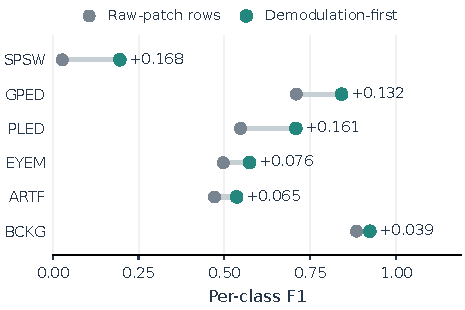
\includegraphics[width=\columnwidth]{figures/class_f1.pdf}
  \caption{\textbf{TUEV gains across event categories.} Paired markers
  compare held-out F1 for raw learned rows and demodulation-first tokens
  with the same reader. Text gives the absolute difference. All six
  categories improve; the figure does not attribute these gains to the
  envelope alone.}
  \label{fig:class}
\end{figure}

\subsection{Where does event recognition improve?}
The aggregate gain extends beyond the majority background category
(\cref{fig:class}). GPED F1 increases from 0.710 to 0.842, and PLED F1
from 0.547 to 0.709. F1 also improves for spike/sharp-wave events, eye
movements, artifacts, and background. These results connect the overall
score to both recurrent-discharge and other event categories, rather
than supporting an explanation confined to a single label type.

The class breakdown also shows what the aggregate metrics hide.
Spike/sharp-wave F1 rises from 0.028 to 0.196, but recall remains 0.109.
For eye movements, F1 improves despite a decline in recall, because
precision rises. Table~\ref{tab:classes} in the appendix reports precision and recall
alongside F1. This distinguishes improved category-level discrimination
from uniform improvements in every operating characteristic.

\section{Discussion and Conclusion}
\label{sec:conclusion}
\paragraph{Scope.}
The matched comparison uses one reader, one seed, and one training recipe. CHB-MIT results describe the specified enriched
window protocol rather than continuous-recording alarm performance.
The filterbank and full-window analytic transform can introduce boundary
and overlap effects; their implementation is documented in the appendix.

\paragraph{Conclusion.}
We construct EEG tokens by pairing local waveform and demodulated
amplitude trajectories before attention. With the reader fixed, this
input improves clinical prediction over raw learned rows; matched
bandwise controls show an advantage over either content view alone.
The result points to a simple design principle: expose useful signal
computations without discarding complementary detail, then let attention
learn their organization.

\section*{LLM Usage Statement}
OpenAI Codex assisted with literature retrieval, manuscript drafting and
editing, code and result-record inspection, figure preparation, and
LaTeX compilation. It also assisted with numerical consistency checks
and the organization of the experimental evidence.

{\small
\bibliographystyle{ieeenat_fullname}
\bibliography{references}
}

\clearpage
\appendix
\section{Data and Evaluation Protocol}
\label{app:data}
\paragraph{TUEV.}
The evaluated TUEV v2.0.1 cache contains five-second windows around
annotated events. Signals are resampled to 200 Hz, bandpass filtered
from 0.3 to 75 Hz, and notch filtered at 60 Hz. Values in microvolts
are divided by 100 before storage. The official training subjects are
sorted and split 80:20 into training and validation partitions; official
evaluation subjects form the test partition. There are 232, 58, and
80 subjects, respectively. We do not apply a second scaling operation
in the model loader.

\paragraph{CHB-MIT.}
The evaluated CHB-MIT v1.0.0 cache resamples the recordings from 256 to
200 Hz and extracts non-overlapping ten-second windows, dropping
incomplete tails. Any overlap with an annotated seizure gives a positive
label. Additional windows are extracted around seizure intervals with
one-second pre/post margins and a five-second stride; these are labeled
positive. This enrichment applies to training, validation, and test
partitions, adding 1,781, 90, and 162 windows, respectively. It is part
of the evaluated protocol, not training augmentation. A natural-grid-only
evaluation would be a different test set.

Each window and channel is divided by its own 95th percentile absolute
amplitude plus $10^{-8}$. Thus amplitude in this experiment refers to
variation within this normalization, not calibrated clinical voltage.
Training uses cases chb01--chb19 and chb21; validation uses chb20 and
chb22; testing uses chb23 and chb24. The repeated-subject recordings
chb01 and chb21 both remain in training. The test set has 17,110 negative
and 276 positive windows (1.59\% positive). PR-AUC should be compared
only on this same case and window composition.

\begin{table}[t]
  \centering
  \caption{\textbf{Evaluated window counts.} Counts include the specified
  CHB-MIT seizure-window enrichment.}
  \label{tab:counts}
  \small
  \begin{tabular}{lrrr}
    \toprule
    Dataset & Train & Validation & Test \\
    \midrule
    TUEV & 68,445 & 15,487 & 29,421 \\
    CHB-MIT & 316,205 & 21,184 & 17,386 \\
    \bottomrule
  \end{tabular}
\end{table}

\paragraph{Common montage.}
Both tasks use the following bipolar chains: FP1--F7--T7--P7--O1,
FP2--F8--T8--P8--O2, FP1--F3--C3--P3--O1, and
FP2--F4--C4--P4--O2. Adjacent pairs in each chain form the 16 channels.
Older T3/T4/T5/T6 aliases are mapped to T7/T8/P7/P8. This is a
16-channel protocol; results from a 23-channel native pipeline require
a separate evaluation rather than direct insertion into the main table.

\paragraph{Metrics.}
For multiclass TUEV, balanced accuracy is mean class recall and weighted
F1 is weighted by test-class support. For binary CHB-MIT, PR-AUC is
trapezoidal integration of the precision--recall curve. Average precision
is also reported because it uses a different interpolation convention.
The binary decision threshold is 0.5. Neither the threshold nor the
checkpoint is selected on test labels.


\begin{table*}[t]
  \centering
  \caption{\textbf{TUEV test-category breakdown.} The two validation-selected
  checkpoints are evaluated on the same 29,421 windows. Bold marks the
  better tokenizer within each class and metric.}
  \label{tab:classes}
  \small
  \begin{tabular}{lrrrrrrr}
    \toprule
    & & \multicolumn{3}{c}{Raw-patch rows} & \multicolumn{3}{c}{\ours{}} \\
    \cmidrule(lr){3-5}\cmidrule(lr){6-8}
    Category & Support & Precision & Recall & F1 & Precision & Recall & F1 \\
    \midrule
    SPSW & 567 & 0.024 & 0.034 & 0.028 & \textbf{0.925} & \textbf{0.109} & \textbf{0.196} \\
    GPED & 4,677 & 0.743 & 0.679 & 0.710 & \textbf{0.915} & \textbf{0.779} & \textbf{0.842} \\
    PLED & 1,998 & \textbf{0.661} & 0.467 & 0.547 & 0.641 & \textbf{0.792} & \textbf{0.709} \\
    EYEM & 329 & 0.396 & \textbf{0.669} & 0.497 & \textbf{0.585} & 0.562 & \textbf{0.574} \\
    ARTF & 2,204 & 0.390 & 0.595 & 0.471 & \textbf{0.463} & \textbf{0.637} & \textbf{0.536} \\
    BCKG & 19,646 & 0.900 & 0.871 & 0.885 & \textbf{0.926} & \textbf{0.922} & \textbf{0.924} \\
    \bottomrule
  \end{tabular}
\end{table*}

\section{Implementation and Training}
\label{app:recipe}
\paragraph{Frontend.}
The 16 sinc filters share their parameters across channels. Each
201-sample symmetric FIR uses a Hamming window and zero padding of
100 samples on each side. The FFT-based Hilbert transform doubles
positive-frequency coefficients, preserves the DC and Nyquist terms,
and zeros negative frequencies. It is applied to the complete 5-s or
10-s filtered window. No extension beyond that window is used for the
analytic transform. Responses near the boundaries may therefore depend
on the finite-window convention.

The initialization is logarithmic; the learned bank is not constrained
to retain constant-Q spacing or non-overlapping passbands. A token
indexes a particular learned filter, rather than presupposing a
physiological frequency category. Each content projection maps 50
samples to 64 coordinates. The envelope projection is affine and has a
learned coordinatewise scale, absorbed into $P_E$ and $\mathbf b_E$ in
\cref{eq:token}. The waveform projection has no bias and is initialized
to zero. Its full trained rank in \cref{tab:rank} confirms that it does
not remain the initial zero map. Content controls preserve these
projection shapes and initialization rules.

\paragraph{Reader.}
Bipolar channel coordinates concatenate the two electrode endpoints
before a two-layer MLP. Dropout acts in the feed-forward sublayer.
Global mean pooling precedes layer normalization and the classifier.

For $C$ channels, $B$ bands, and $P$ intervals, the number of attention
scores per head and block is
\begin{equation}
  CBP^2+BP C^2+CP B^2=CBP(P+C+B).
  \label{eq:complexity}
\end{equation}
This describes attention-score complexity, not measured throughput.
Projection and feed-forward costs remain proportional to token count
and feature dimension. TUEV has $16\times16\times20=5{,}120$ tokens;
CHB-MIT has $16\times16\times40=10{,}240$.



\paragraph{Training augmentation.}
One of five transformations is sampled uniformly per training batch:
time reversal with probability 0.5, Gaussian noise with standard
deviation 0.05 in stored signal units, masking 20\% of temporal samples,
masking 20\% of channels, or masking Fourier bins with probability 0.2.
Transformations act on the input before either frontend. The raw-row
and band-content arms use the same choices. No training augmentation
is applied during validation, testing, or token recovery.

\paragraph{Checkpoint selection.}
TUEV is validated once per epoch. CHB-MIT is validated every 200
optimizer steps and at epoch end. The patience counter counts
non-improving validation evaluations; the stopping condition is checked
at epoch boundaries. Patience is 20 for both tasks. The completed TUEV
models finish all 20 epochs, whereas the CHB-MIT reference stops by
patience after four epochs. Neither reported reference is terminated
by its wall-clock budget. The selected TUEV reference checkpoint comes
from evaluation 1 (zero-based), and the raw-row checkpoint from
evaluation 14; the CHB-MIT reference comes from evaluation 130.
The new TUEV waveform-only and envelope-only controls also select
evaluation 1 and complete all 20 epochs. The CHB-MIT raw-row control
selects evaluation 246 and stops by patience after six epochs.
All selection uses the validation metric specified in \cref{sec:setup}.

\paragraph{Exploratory representation controls.}
The mean-envelope control replaces each 50-sample log1p-envelope patch
by its within-patch mean, repeated 50 times. Filtering, the full-window
Hilbert transform, both projection matrices, their initialization, and
the waveform input remain unchanged. The bandmix control multiplies
the 16-band token axis by a fixed dense orthogonal matrix obtained by QR
factorization of a Gaussian matrix with seed 2. The same matrix acts on
all channels, intervals, features and examples, before positional
embeddings. It adds no trainable parameters. Each control changes one
model configuration field relative to the paired reference. The
mean-envelope arm reaches $\kappa=0.695$, retaining amplitude changes
between token intervals while averaging variation within each interval.
The mixed-basis arm reaches 0.585. These supplementary comparisons are
reported in \cref{tab:content-metrics}; the main content comparison
holds the physical grid fixed.

\paragraph{Complete content-control metrics.}
\label{app:content-metrics}
\Cref{tab:content-metrics} reports all three task metrics for the completed
comparisons. Each row uses the test predictions of its validation-selected
checkpoint. The CHB-MIT raw-row and paired models have average precision
0.642 and 0.702, respectively. Original prediction and checkpoint hashes
are retained with the result records.

\begin{table}[t]
  \centering
  \caption{\textbf{Complete metrics for the content comparisons.}
  Seed 2 throughout. The two CHB-MIT rows use the same enriched
  17,386-window test protocol. Bold denotes the best value per panel.}
  \label{tab:content-metrics}
  \small
  \begin{tabular}{lrrr}
    \toprule
    TUEV input & $\kappa$ & Bal. acc. & wF1 \\
    \midrule
    Waveform only & 0.498 & 0.510 & 0.735 \\
    Envelope only & 0.642 & 0.577 & 0.812 \\
    Envelope + waveform & \textbf{0.711} & \textbf{0.634} & \textbf{0.849} \\
    Waveform + mean E & 0.695 & 0.612 & 0.842 \\
    Mixed band basis & 0.585 & 0.530 & 0.788 \\
    \midrule
    CHB-MIT input & PR-AUC & AUROC & Bal. acc. \\
    \midrule
    Raw learned rows & 0.642 & \textbf{0.928} & 0.538 \\
    Envelope + waveform & \textbf{0.699} & 0.918 & \textbf{0.630} \\
    \bottomrule
  \end{tabular}
\end{table}

\section{Recoverability of Paired Content}
\label{app:recovery}
\paragraph{Why reconstruction is possible.}
Write a token before positional embeddings as
$\mathbf h=[P_E\boldsymbol\ell+\mathbf b_E;P_W\mathbf w]$, where
$\boldsymbol\ell=\log(1+\mathbf e)$. If both projection matrices have
column rank $L$, their Moore--Penrose inverses recover the two local
input vectors in exact arithmetic:
\begin{equation}
  \boldsymbol\ell=P_E^{\dagger}(\mathbf h_E-\mathbf b_E),\qquad
  \mathbf w=P_W^{\dagger}\mathbf h_W.
  \label{eq:inverse}
\end{equation}
Interleaving token coordinates merely changes how the two blocks are
indexed. The envelope follows by applying $\exp(\boldsymbol\ell)-1$.
This statement concerns the band-limited waveform and its envelope;
it is not a claim that the complete original recording can be inverted
from the filterbank.

\begin{table}[t]
  \centering
  \caption{\textbf{Trained projection matrices.} Each matrix has shape
  $64\times50$. Full column rank explains local recoverability;
  conditioning determines sensitivity to numerical error.}
  \label{tab:rank}
  \small
  \begin{tabular}{llrr}
    \toprule
    Dataset & Projection & Rank & Condition no. \\
    \midrule
    TUEV & Waveform & 50 & $3.90\times10^4$ \\
         & Log-envelope & 50 & $11.66$ \\
    CHB-MIT & Waveform & 50 & $3.25\times10^4$ \\
            & Log-envelope & 50 & $11.64$ \\
    \bottomrule
  \end{tabular}
\end{table}

\paragraph{Readout protocol.}
For each dataset we select 128 training, 32 validation, and 64 test
windows with fixed seed 2. Four evenly spaced channel indices, all 16
bands, and three fixed interior patch indices are used per window.
The sample counts for fitting, validation, and testing are consequently
24,576, 6,144, and 12,288 tokens. Separate ridge readouts predict the
50 waveform or log-envelope samples from the 128 token coordinates.
Each readout is shared across channel, band, and patch indices.
The regularization coefficient is selected from
$\{10^{-8},10^{-5},10^{-2},1\}$ by validation reconstruction error;
both datasets select $10^{-8}$ for both targets.

Token coordinates are standardized with training-set means and standard
deviations before fitting each ridge readout. Normalized RMSE is the
square root of the total squared prediction error divided by the target's
summed squared deviations from its per-coordinate test-set mean.
For the physical envelope, obtained by exponentiating the log-envelope
prediction, normalized RMSE is $1.12\times10^{-6}$ on TUEV and
$1.38\times10^{-6}$ on CHB-MIT. A second check using the known projection
weights and \cref{eq:inverse} produces the same qualitative result.
Figure~\ref{fig:recovery} shows a fixed example, not a reconstruction
chosen to minimize error: the first held-out window and selected channel,
band 12, and the middle of the three sampled intervals.

\paragraph{What a linear patch map cannot compute.}
For a nonzero filtered signal $w$, its envelope satisfies
$|\mathcal A(-w)|=|\mathcal A(w)|$, where $\mathcal A$ is the linear
analytic-signal operator. A linear map instead satisfies
$F(-w)=-F(w)$. It therefore cannot equal the nonzero envelope map for
both $w$ and $-w$. This does not imply that a linear token loses the
waveform, or that a nonlinear encoder cannot learn to compute an
envelope. It identifies the computation explicitly moved ahead of the
encoder in our representation.

\paragraph{Event categories.}

SPSW denotes spike and sharp waves, GPED generalized periodic epileptiform
discharges, PLED periodic lateralized epileptiform discharges, EYEM eye
movement, ARTF artifact, and BCKG background.


\section{Historical Baseline Configurations}
\label{app:baselines}
\paragraph{Runs and initialization.}
The main table reuses complete baseline result records on the shared
16-channel protocols. Each multi-run cell includes all three recorded
seeds from one training recipe. The TUEV LaBraM and EEGPT entries use
single completed runs through the authors' shared16 entrypoints, with
scratch and pretrained initialization reported separately. The older
LaBraM results on 26,067 evaluation windows are outside this comparison.
CHB-MIT scratch EEGPT and REVE have no completed result on the evaluated
17,386-window protocol, so those cells remain empty. TFM's main-table
entry uses both its pretrained tokenizer and pretrained encoder.

\paragraph{Task adaptations.}
Historical baselines retain their recorded, model-specific recipes.
BIOT uses its channelwise spectral input. The historical CBraMod
implementation uses an 800-unit local classification head; its binary
variant uses two logits and focal loss. CHB-MIT EEGPT uses a decoder
derived from its sleep-stage configuration and a 16-to-19 channel
mapping. The recorded REVE implementation uses direct fine-tuning with
AdamW and omits the native learned-query context token. These scores
therefore describe the documented task adaptations rather than exact
reproductions of every model's published training pipeline. Their
optimizer, loss, batch size, and training budget are preserved in the
accompanying result records. The matched-reader comparison in
\cref{tab:fixed-reader} instead uses the same recipe in both arms.

\paragraph{Metrics and model size.}
The shared evaluation uses trapezoidal PR-AUC and a fixed binary threshold
of 0.5. The native LaBraM keys \texttt{balanced\_accuracy} and
\texttt{f1\_weighted} map to balanced accuracy and weighted F1.
Model sizes include task-specific heads and can differ between datasets:
for example, the recorded CBraMod instances contain 17.85M parameters
on TUEV and 30.65M on CHB-MIT. Total parameter counts were not retained
for the native shared16 LaBraM and EEGPT runs; the table leaves those
sizes unreported rather than borrowing counts from different heads.

\end{document}
